\section{Experiments}
\label{sec:experiments}

\subsection{Setup and Research Questions}
\label{sec:setup}

We evaluate QKFormer~\cite{zhou2024qkformer} on CIFAR-10 and CIFAR-100 at
$T=1$ and $T=4$. Address reconstruction uses disjoint calibration and
validation data. Unless stated otherwise, current replacement uses a seed-42
checkpoint, 128 training batches for calibration, and the complete validation
split. Existing seed-43/44 runs are used only where they were already completed
as robustness evidence.

The experiments answer five questions:
\begin{itemize}
  \item \textbf{RQ1}: Do Q/K spike states carry address-specific response
  information beyond coarse state, smoothing, and table capacity?
  \item \textbf{RQ2}: Can unsupported addresses be handled transparently
  rather than hidden as successful lookups?
  \item \textbf{RQ3}: Can semantic subspaces preserve the useful signal with a
  smaller supported-entry budget?
  \item \textbf{RQ4}: Does temporal-channel calibration preserve end-to-end
  behavior after local response lookup?
  \item \textbf{RQ5}: Is lookup fidelity conditioned on the attention
  interaction, and where does the current replacement boundary lie?
\end{itemize}
Historical experiment identifiers E0, E1, E5, and E7 are retained in captions
for traceability, but the presentation follows these research questions.

\subsection{Main Result: End-to-End Lookup Fidelity}
\label{sec:main_fidelity}

Table~\ref{tab:main_fidelity} separates completed QKFormer measurements from
registered but unfinished dataset extensions. The completed rows replace the
\texttt{stage1.0.tssa} current. Static semantic lookup can already be close on
CIFAR-10, but it collapses by 13.07 points on CIFAR-100 $T=4$. TCSLU reduces
the worst completed loss to 0.44 points. The $+0.11$ CIFAR-10 $T=4$
difference is treated as no-loss fluctuation rather than an accuracy gain.

\begin{table*}[t]
\centering
\footnotesize
\setlength{\tabcolsep}{5pt}
\begin{tabular}{llrrrrl}
\toprule
Architecture / dataset & $T$ & Clean & Static LUT & TCSLU & Drop & Status \\
\midrule
QKFormer / CIFAR-10  & 1 & 94.64 & 93.64 & 94.57 & 0.07 & Complete \\
QKFormer / CIFAR-10  & 4 & 95.70 & 95.08 & 95.81 & -0.11 & Complete \\
QKFormer / CIFAR-100 & 1 & 77.69 & 75.94 & 77.57 & 0.12 & Complete \\
QKFormer / CIFAR-100 & 4 & 81.09 & 68.02 & 80.65 & 0.44 & Complete \\
\midrule
QKFormer Route 1 / CIFAR10-DVS & 16 & 82.30 & -- & 83.90 & -1.60 &
Complete below gate \\
SpiLiFormer Route 3 / CIFAR10-DVS & 16 & 81.20 & -- & 81.70 & -0.50 &
Complete boundary \\
QKFormer / ImageNet-100 & \tbd & \tbd & \tbd & \tbd & \tbd & Pending \\
Mini-QKFormer / DVS128 Gesture & 16 & 98.61 & \tbd & \tbd & \tbd &
Backbone only \\
\bottomrule
\end{tabular}
\caption{End-to-end lookup-fidelity matrix (Acc@1, \%). Drop is clean minus
TCSLU or the registered LUT-only deployment; negative values are no-loss
fluctuations. All completed rows use full validation. CIFAR10-DVS uses 1,000
samples and bypasses the replaced original projection. ImageNet-100 remains a
placeholder. The DVS128 value is a reproduced backbone baseline and does not
yet contain LUT replacement.}
\label{tab:main_fidelity}
\end{table*}

The CIFAR10-DVS route history requires a qualification. In the original fixed
queue, Route 3 was not launched because the official SpiLiFormer release did
not provide a CIFAR10-DVS checkpoint. A later user-authorized extension trained
SpiLiFormer-2-256 from scratch for 130 effective epochs and then completed the
fixed 12-epoch LUT transfer. The clean model reached $81.2\%$ at epoch 103,
not the published $86.7\%$; the LUT-only deployment reached $81.7\%$ at epoch
7, a paired $+0.5$-point change. Route 1 remains the best valid event-data
deployment at $83.9\%$. Neither route crosses the registered $84.0\%$ gate.

\subsection{RQ1: Does the Address Carry Semantics?}
\label{sec:address_semantics}

\paragraph{Occupancy and conditional structure (E0).}
Table~\ref{tab:e0_feasibility} reports address coverage, singleton fraction,
and response variance within addresses. The address spaces remain populated
across datasets and time steps; the result motivates held-out testing but is
not itself evidence that the address semantics are correct.

\begin{table}[t]
\centering
\footnotesize
\resizebox{\columnwidth}{!}{%
\begin{tabular}{lccc}
\toprule
Setting & Coverage & Singleton frac. & Cond. var. \\
\midrule
CIFAR-10 $T=4$ & 0.5993 & 0.0865 & 0.0713 \\
CIFAR-10 $T=1$ & 0.5805 & 0.0794 & 0.0549 \\
CIFAR-10 $T=1$, seed 43 & 0.5789 & 0.0822 & 0.0498 \\
CIFAR-10 $T=1$, seed 44 & 0.5840 & 0.0805 & 0.0529 \\
CIFAR-100 $T=1$ & 0.5900 & 0.0768 & 0.0747 \\
CIFAR-100 $T=4$ & 0.6128 & 0.0790 & 0.0894 \\
\bottomrule
\end{tabular}
}
\caption{E0 feasibility diagnostics. Coverage measures occupied mixed-radix
addresses; it is not a hash-collision statistic. Conditional variance measures
response dispersion within an address.}
\label{tab:e0_feasibility}
\end{table}

\paragraph{Held-out reconstruction (E1).}
Correct Q/K addresses reduce response MSE by $3.71\%$ on CIFAR-10 and
$4.42\%$ on CIFAR-100 relative to a global mean. Coarse token/channel lookup
explains part, but not all, of the effect. Candidate/background means are nearly
identical to the global baseline, while shuffling the address--prototype map
makes reconstruction substantially worse.

\begin{table}[t]
\centering
\footnotesize
\resizebox{\columnwidth}{!}{%
\begin{tabular}{lrrrr}
\toprule
Dataset & Token/channel & Address & Candidate/back. & Shuffled \\
\midrule
CIFAR-10 & 2.7941 & \textbf{3.7080} & 0.0329 & -17.8260 \\
CIFAR-100 & 3.4246 & \textbf{4.4247} & 0.0356 & -15.8216 \\
CIFAR-100 $T=4$ & 2.24 & \textbf{2.84} & 0.02 & -13.74 \\
\bottomrule
\end{tabular}
}
\caption{E1 held-out relative MSE reduction (\%) against the global mean.
Correct addresses outperform coarse lookup, while shuffled assignment preserves
table capacity but destroys the gain.}
\label{tab:e1_recon}
\end{table}

\begin{figure*}[t]
  \centering
  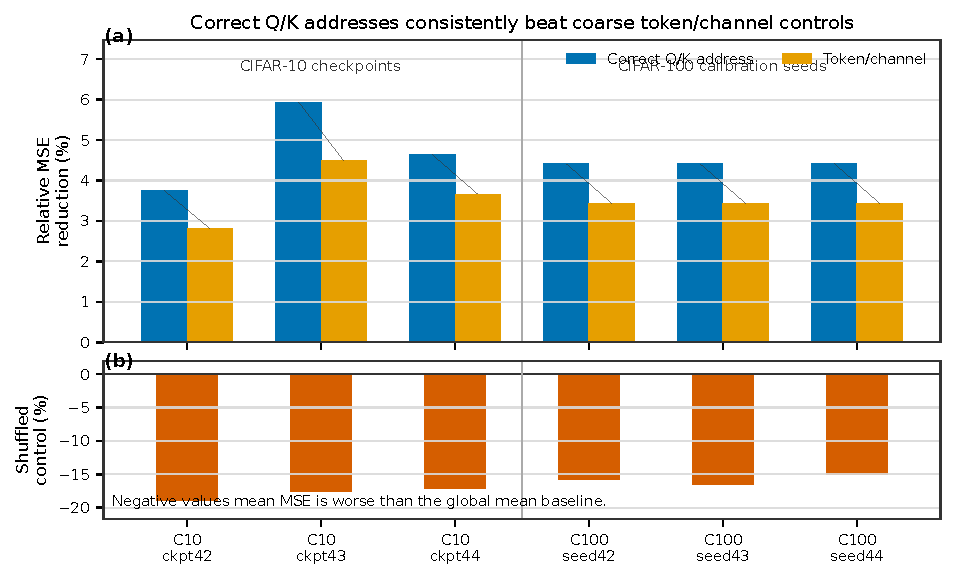
\includegraphics[width=\textwidth]{figures/fig3_e1_reconstruction.pdf}
  \caption{Held-out address controls. Correct Q/K addresses outperform
  token/channel lookup across independently trained CIFAR-10 checkpoints and
  CIFAR-100 calibration subsets. Shuffled address assignment falls below the
  global baseline, isolating alignment from table capacity.}
  \label{fig:e1-reconstruction}
\end{figure*}

The result also holds on independently trained CIFAR-10 $T=1$ checkpoints:
address reductions are $3.7597\%$, $5.9361\%$, and $4.6503\%$ for seeds
42--44, exceeding token/channel by an average of 1.1318 percentage points.
Across five fixed CIFAR-10 $T=4$ calibration subsets, aligned TCSLU ranks first
in all five. Its paired advantages over global and token/channel controls are
$+0.190$ and $+0.278$ points, with 95\% intervals
$[+0.037,+0.343]$ and $[+0.014,+0.542]$, respectively.

\begin{table}[t]
\centering
\footnotesize
\resizebox{\columnwidth}{!}{%
\begin{tabular}{llcc}
\toprule
Setting & Control & Static LUT & TCSLU \\
\midrule
CIFAR-10 $T=4$ & Aligned Q/K & \textbf{95.08} & \textbf{95.81} \\
 & Global mean & 91.41 & 95.63 \\
 & Same-size random & 91.87 & 95.52 \\
 & Token/channel & 94.86 & 95.45 \\
 & Shuffled Q/K & 90.57 & 95.31 \\
\midrule
CIFAR-100 $T=1$ & Aligned Q/K & \textbf{75.94} & \textbf{77.57} \\
 & Global mean & 73.05 & 77.37 \\
 & Same-size random & 72.74 & 76.63 \\
 & Token/channel & 75.50 & 76.35 \\
 & Shuffled Q/K & 73.00 & 76.43 \\
\bottomrule
\end{tabular}
}
\caption{Matched semantic controls for stage1 current replacement (Acc@1,
\%). Checkpoint, calibration budget, target, validation split, and table size
are fixed within each setting.}
\label{tab:current_replacement_controls}
\end{table}

\subsection{RQ2: Support, Sparsity, and Global Backoff}
\label{sec:support_backoff_results}

The mixed-radix encoding has no tuple-level hash collision. The practical
questions are whether quantization aliases responses and whether calibration
provides enough support. At eight CIFAR-100 calibration batches, the correct
address already reduces MSE by $3.7840\%$, compared with $3.3258\%$ for
token/channel, and the validation hit rate is $99.7982\%$. At 128 batches the
hit rate reaches $99.9907\%$.

\begin{figure}[t]
  \centering
  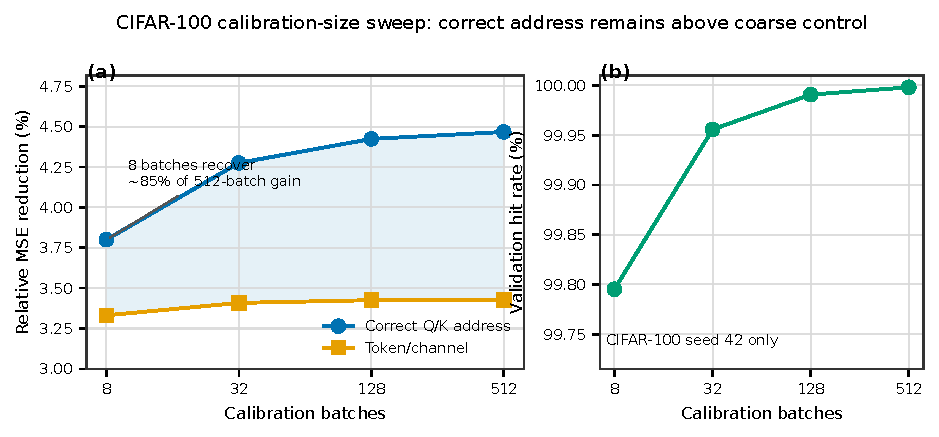
\includegraphics[width=\columnwidth]{figures/fig4_calibration_sweep.pdf}
  \caption{Calibration efficiency. Correct addresses remain above
  token/channel lookup from 8 to 512 calibration batches, while validation hit
  rate saturates. Curves average calibration seeds 42--44.}
  \label{fig:calibration-sweep}
\end{figure}

The E5 hierarchy records every fallback level and assigns no validation
response to an unsupported fine address. From eight batches onward, it beats
token/channel for every completed seed and retains at least $80\%$ of the
full-address gain. This is a successful reliability mechanism but only a
partial compactness result: its effective supported entries grow from
$40.4\%$ to $51.1\%$ of the compact full-address space.

\begin{table}[t]
\centering
\footnotesize
\resizebox{\columnwidth}{!}{%
\begin{tabular}{rcccc}
\toprule
Calib. & Hierarchy & Full addr. & Token/ch. & Eff. entries \\
\midrule
1 & 0.3178 & 0.4179 & 2.5493 & 0.3305 \\
8 & 3.7742 & 3.7840 & 3.3258 & 0.4040 \\
32 & 4.2667 & 4.2671 & 3.4027 & 0.4477 \\
128 & 4.4248 & 4.4247 & 3.4246 & 0.4822 \\
512 & 4.4752 & 4.4752 & 3.4386 & 0.5107 \\
\bottomrule
\end{tabular}
}
\caption{E5 support-aware backoff on CIFAR-100 $T=1$. Reconstruction columns
are relative MSE reductions (\%) averaged over calibration seeds 42--44.
Effective entries are normalized by the compact full-address space.}
\label{tab:e5_backoff}
\end{table}

\subsection{RQ3: Compactness Through Subspace Decoupling}
\label{sec:subspace_results}

E7 addresses the compactness limit of the hierarchy. In the fixed CIFAR-100
$T=1$, seed-42, 128-batch analysis, TC+Q/gate retains $87.58\%$ of the
full-address gain with $8.83\%$ of the compact address-space entries. TC+QK
retains $94.31\%$ with $20.54\%$. Both remain below the predeclared 25\%
entry gate and both matched shuffled-subspace controls are worse than the
global mean.

\begin{table}[t]
\centering
\footnotesize
\resizebox{\columnwidth}{!}{%
\begin{tabular}{lrrrrrr}
\toprule
Estimator & Red. & Shuf. & Entries & Frac. & Ret. & Meta. KiB \\
\midrule
Token/channel & 3.4253 & -- & 2,052 & 2.95 & 77.42 & 20.29 \\
TC+Q/gate & 3.8749 & -1.8908 & 6,148 & 8.83 & 87.58 & 60.79 \\
TC+QK & 4.1727 & -1.6600 & 14,303 & 20.54 & 94.31 & 141.42 \\
Full address & 4.4243 & -- & 19,258 & 27.66 & 100.00 & 190.42 \\
\bottomrule
\end{tabular}
}
\caption{E7 subspace ablation. Reduction, shuffled control, entry fraction,
and gain retention are percentages. Metadata-aware KiB uses sparse FP32
values, uint32 keys, uint16 counters, and validity bits; it remains an
analytical proxy rather than measured memory.}
\label{tab:e7_subspace}
\end{table}

\begin{figure*}[t]
  \centering
  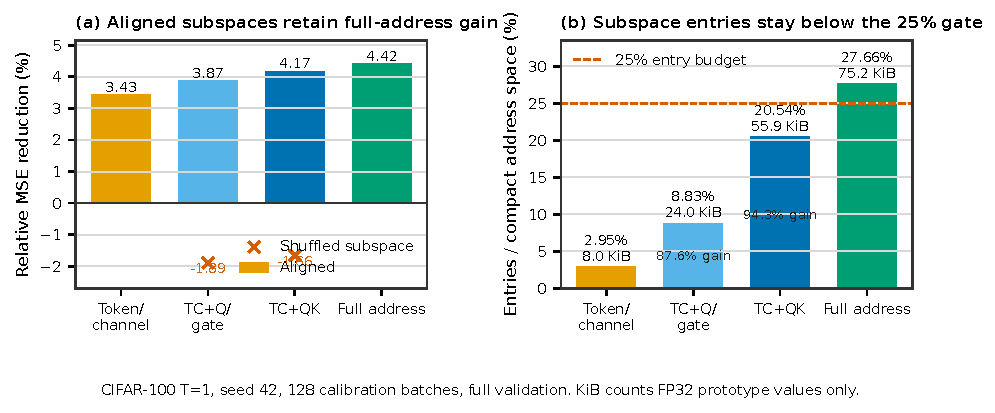
\includegraphics[width=\textwidth]{figures/fig5_e7_component_ablation.pdf}
  \caption{E7 component ablation. Aligned semantic subtables retain most
  full-address reconstruction gain below the 25\% entry gate, while matched
  shuffled subtables fall below the global baseline.}
  \label{fig:e7-component}
\end{figure*}

\subsection{RQ4: Why TCSLU Works}
\label{sec:tcslu_results}

Table~\ref{tab:tcslu_ablation} separates static lookup from calibration
components. Temporal-only matching is insufficient and can be destructive,
especially at $T=4$. Channel-conditioned or joint moment matching restores
most of the lost accuracy. In the current implementation, the TCSLU row shares
the calibrated time/channel moment transform with the strongest moment row and
adds the explicit support-aware lookup contract; it should not be interpreted
as an independently tuned accuracy booster.

\begin{table}[t]
\centering
\footnotesize
\resizebox{\columnwidth}{!}{%
\begin{tabular}{lrr}
\toprule
Variant & CIFAR-100 $T=1$ & CIFAR-100 $T=4$ \\
\midrule
Clean & 77.69 & 81.09 \\
Static semantic LUT & 75.94 & 68.02 \\
Temporal-only match & 64.02 & 46.97 \\
Channel-only match & 77.57 & 80.15 \\
Moment match & 77.57 & 80.65 \\
TCSLU + backoff & \textbf{77.57} & \textbf{80.65} \\
\bottomrule
\end{tabular}
}
\caption{TCSLU component study (Acc@1, \%). The result supports dynamic
current calibration, not a claim that each named component produces an
independent monotonic gain.}
\label{tab:tcslu_ablation}
\end{table}

The semantic control remains necessary after calibration
(Table~\ref{tab:current_replacement_controls}), so TCSLU is not merely generic
smoothing. The combined interpretation is that the address retrieves a
response mode while calibration restores the statistics required by the
downstream BN/LIF path.

\subsection{RQ5: Robustness and Contract-Conditioned Transfer}
\label{sec:robustness_transfer}

QKFormer robustness checks preserve the same scoped conclusion. Minimum
support thresholds 1, 2, and 4 produce the same $95.81\%$ CIFAR-10 $T=4$
result under the dense 2,048-entry calibration regime. Replacing stage1 and
stage2 together gives $95.43\%$ from a $95.70\%$ clean baseline, whereas the
static LUT falls to $88.99\%$. Under noise and brightness severity 1, TCSLU
differs from the corresponding clean-hook model by 0.01 and 0.06 points.

\begin{table*}[t]
\centering
\footnotesize
\resizebox{\textwidth}{!}{%
\begin{tabular}{llrrrrl}
\toprule
Architecture & Intervention & Clean & Static & Calibrated & Drop & Interpretation \\
\midrule
QKFormer & CIFAR-10 $T=4$, stage1 & 95.70 & 95.08 & 95.81 & -0.11 &
Native positive setting \\
QKFormer & CIFAR-10 $T=4$, stage1+2 & 95.70 & 88.99 & 95.43 & 0.27 &
Scope robustness \\
Spikformer & Original SSA current & 88.16 & 66.47 & 76.35 & 11.81 &
Contract mismatch \\
QK-contract Spikformer & $\operatorname{gate}(Q)\odot K$ SSA & 87.54 & 81.53 &
86.16 & 1.38 & Structure-conditioned recovery \\
QKFormer Route 1 & CIFAR10-DVS LUT-only stage1 & 82.30 & -- & 83.90 & -1.60 &
Best event deployment; below gate \\
SpiLiFormer Route 3 & CIFAR10-DVS first FF-LiDiff & 81.20 & -- & 81.70 & -0.50 &
Executable cross-architecture boundary \\
\bottomrule
\end{tabular}
}
\caption{Robustness and contract intervention (Acc@1, \%). The modified
Spikformer row is an architecture ablation, not evidence that unmodified
Spikformer is near-losslessly replaced. Under matched controls it reaches
85.83 with shuffled address and 86.18 with token/channel, so fine-address
superiority beyond coarse state remains unresolved.}
\label{tab:contract_transfer}
\end{table*}

Changing Spikformer to a QKFormer-like interaction recovers 88.3\% of the
original replacement gap while preserving clean accuracy within 0.62 points.
This supports the interaction contract as a condition for lookup compatibility.
It does not establish a general principle for all spiking neurons or all
Spiking Transformer families.

The CIFAR10-DVS routes add bounded implementation evidence. Both accepted
deployments use all 1,000 validation samples, trainable per-time/per-channel
current normalization, and a module that does not retain or execute the
replaced \texttt{proj\_conv}. Route 3 shows that the first FF-LiDiff LUT path
can match and slightly exceed its paired from-scratch SpiLiFormer teacher.
Its absolute accuracy is limited by the failed clean-backbone reproduction,
and Route 1's $83.9\%$ remains the strongest event-data result.

\subsection{Replacement Completeness Boundary}
\label{sec:replacement_boundary}

Table~\ref{tab:replacement_boundary} compresses the operator-completeness
studies into one boundary view. The semantic TCSLU result is compact but local.
The grouped projection and native operator audits broaden the replaced scope,
but they are fidelity studies with larger tables and do not establish hardware
efficiency.

\begin{table*}[t]
\centering
\footnotesize
\resizebox{\textwidth}{!}{%
\begin{tabular}{p{0.18\textwidth}p{0.24\textwidth}p{0.14\textwidth}p{0.13\textwidth}p{0.26\textwidth}}
\toprule
Audit & Replaced scope & Worst completed drop & Reported footprint &
What remains outside the claim \\
\midrule
TCSLU semantic current & One or two early attention currents &
0.44 pp & 8.0 KiB prototype values &
Other currents, operators, memory hierarchy, and measured execution \\
Grouped 2-bit projection LUT & All four attention \texttt{proj\_conv} currents &
0.06 pp & 2,664 KiB FP32 values &
Q/K/V, MLP, patch embedding, BN/LIF, and runtime removal in the hook study \\
Native affine/BN/LIF LUT & 32 affine operators, 31 paired BN modules, 35 LIF transitions &
0.22 pp & 16,980 KiB LIF values at $T=4$; affine tables additional &
Pooling, residual addition, SSA products/gating, global reductions, hardware cost \\
\bottomrule
\end{tabular}
}
\caption{Replacement-completeness boundary. Footprints are analytical table
values, not measured SRAM or GPU memory. Detailed grouped and native operator
constructions are provided in Appendix~\ref{sec:supp_replacement}.}
\label{tab:replacement_boundary}
\end{table*}

Overall, the core evidence establishes semantic lookup-addressability,
transparent support handling, compact subspace composition, and calibrated
current fidelity under QK-compatible contracts. It does not establish measured
latency, energy, SRAM, ImageNet performance, an event-data result above the
registered 84.0\% gate, unrestricted cross-architecture replacement, or a
complete production full-graph wrapper.
